% =====================================================================
% PARTIE 7 : LA COMMANDE ET L'INFORMATIQUE (etude informatique v2.4, texte integral)
\clearpage
\partieENO{La commande et l'informatique}

Cette partie reprend en entier l'étude informatique de la tour : la commande automatique, l'accès à distance, la mise en service et les premières mesures réelles. Au départ, le Raspberry lit déjà la sonde pH et la batterie par l'intermédiaire de l'Arduino, mais la pompe ne se commande qu'à la main depuis le dashboard : la tour mesure, mais n'agit pas seule. Pour la rendre autonome, il faut qu'un programme prenne lui-même les décisions : quand arroser, quand ajouter de l'engrais, quand économiser la batterie.

Je commence par présenter le système (8.1), puis le matériel et le câblage (8.2). Je décris ensuite le programme de l'Arduino (8.3) et celui du Raspberry Pi (8.4), puis le dashboard (8.5). Je traite l'accès à distance et la sécurité (8.6), la mise en service sur le matériel (8.7) et les premières mesures réelles (8.8). Je termine par les essais (8.9), la synthèse (8.10), l'organisation des fichiers (8.11) et un rappel de la première version du programme (8.12). La fabrication de la sonde EC fait l'objet de la partie 7, et le dashboard de démonstration celui de la partie 9.

\begin{attention}
Le schéma officiel de la carte Arduino Uno, qui donne les noms des broches, est reproduit ci-dessous (il est aussi dans l'Annexe 5, à la fin du rapport). Pour bien lire les parties 7 à 9, trois points. Premièrement, ces parties décrivent le système final, mais le montage réel avance par étapes : les captures, les valeurs d'exemple et les relevés des parties 8.5 à 9 viennent d'un Arduino simulé ou des premières mesures réelles de la partie 8.8, et le tableau de synthèse (8.10) dit, fonction par fonction, ce qui est vérifié sur le matériel. Deuxièmement, la sonde EC du système final est la sonde fabriquée de la partie 7, lue directement par l'Arduino (broches D5, D6 et A0) avec sa propre constante $K$ ; la sonde du commerce (DFRobot DFR0300, $K = 1$, lue par l'ADS1115\ix{16}) était celle du système de départ, et seul l'exemple de la partie 8.4 en garde la trace. Troisièmement, au début le pH est lu directement par l'entrée A1 de l'Arduino ; dans le montage final, il l'est par l'ADS1115\ix{16} (entrée A0), plus précis.
\end{attention}

\schemapaysageC[page=1]{A000066-schematics.pdf}{uno1}{Schéma électrique officiel de la carte Arduino Uno Rev3 (référence A000066), publié par le constructeur : alimentation, microcontrôleur et liaison USB. Les noms des broches (D5, D6, A0, A4, A5...) servent de repère pour lire les feuilles de commande de la partie 8.2.}
\schemapaysageC[page=2]{A000066-schematics.pdf}{uno2}{Schéma électrique officiel de la carte Arduino Uno Rev3 (suite) : les connecteurs.}

% ---------------------------------------------------------------------
\Needspace{8\baselineskip}\subsection{Présentation du système}

Avant d'entrer dans le détail des choix, cette sous-partie présente chaque élément du système, pour qu'on sache de quoi il est fait et à quoi il sert. Elle commence par ce que le programme doit faire, sous forme de cinq missions, puis explique pourquoi je confie les décisions au Raspberry et l'exécution à l'Arduino. Après une vue d'ensemble du système, elle détaille chaque élément : les cartes électroniques, les capteurs, les pompes et les programmes. Elle présente ensuite le serveur, qui fait tourner la tour, et le dashboard, qui permet de la surveiller de près comme de loin, avant d'expliquer pourquoi certaines mesures doivent être faites en alternance.

\subsubsection*{Ce que fait le programme}

Avant d'écrire une ligne de code, je liste ce que la tour doit faire seule. J'en tire cinq missions, qui servent de cahier des charges pour toute la suite : chaque partie du programme répond à l'une d'elles. Je mets la protection au même niveau que l'arrosage, car une pompe qui tourne à sec ou une batterie vidée à fond peuvent abîmer le matériel pour de bon.

\begin{itemize}
\item \textbf{Mesurer} toutes les 10 secondes : pH, conductivité (EC), températures de l'eau et de l'air, humidité, pression, lumière, niveau du réservoir et état de la batterie.
\item \textbf{Arroser} : la pompe principale tourne par cycles (\qty{15}{min} de marche, \qty{15}{min} d'arrêt par défaut).
\item \textbf{Nourrir} : les pompes doseuses ajoutent l'engrais A, l'engrais B ou le correcteur pH$-$ par petites doses, selon le légume cultivé et son stade.
\item \textbf{Protéger} la batterie, la pompe et les plantes : coupure quand la batterie est basse, arrêt quand le réservoir est presque vide, nombre de doses limité.
\item \textbf{Montrer} tout cela sur un dashboard web, consultable depuis la maison ou depuis Internet après connexion, et sur le petit écran de la tour.
\end{itemize}

\subsubsection*{Le Raspberry décide, l'Arduino exécute}

J'ai deux cartes à disposition : le Raspberry Pi et l'Arduino Uno. J'hésite entre deux solutions : écrire tout le programme dans l'Arduino, ou ne lui laisser que la lecture des capteurs et la commande des pompes. L'Arduino a des entrées analogiques et supporte bien le \qty{5}{V}, mais il a peu de mémoire, pas d'heure fiable, ni base de données ni réseau. Le Raspberry, lui, fait tourner Python, garde l'historique et sert le dashboard. Je choisis donc de mettre toute l'intelligence dans le Raspberry, et de garder le protocole Firmata déjà utilisé dans le projet, pour ne jamais avoir à reprogrammer l'Arduino quand je change une règle.

L'Arduino est relié aux capteurs et aux pompes : ce sont les « yeux et les mains » de la tour. Le Raspberry Pi est le « cerveau » : il reçoit les mesures, décide de ce qu'il faut faire, enregistre l'historique et fait tourner le dashboard. Les deux cartes se parlent par le câble USB avec le protocole Firmata.

\begin{aretenir}
L'Arduino ne prend aucune décision, sauf une : si le Raspberry se tait pendant 30 secondes, il coupe toutes les pompes par sécurité (partie 8.3). Il ne surveille pas encore le niveau d'eau lui-même : c'est le Raspberry qui le fait.
\end{aretenir}

\subsubsection*{Vue d'ensemble}

Avant de câbler, je dessine l'ensemble du système pour vérifier que chaque élément a sa place et qu'aucune liaison n'est oubliée. Je le présente sous la forme d'un schéma synoptique normalisé (IEC 61082-1) : chaque élément est un bloc portant un repère selon IEC 81346, dont la lettre indique la fonction (G : production d'énergie, T : conversion, C : stockage, F : protection, K : traitement de l'information, B : capteur, Q : commutation de puissance, M : entraînement, P : affichage). Les traits forts portent l'énergie, les traits fins les signaux, et les symboles du panneau, du convertisseur, de la batterie, du fusible et des moteurs sont ceux de la norme IEC 60617. Les sous-parties suivantes présentent ces éléments un par un, en reprenant leurs repères.

\begin{figure}[H]
\centering
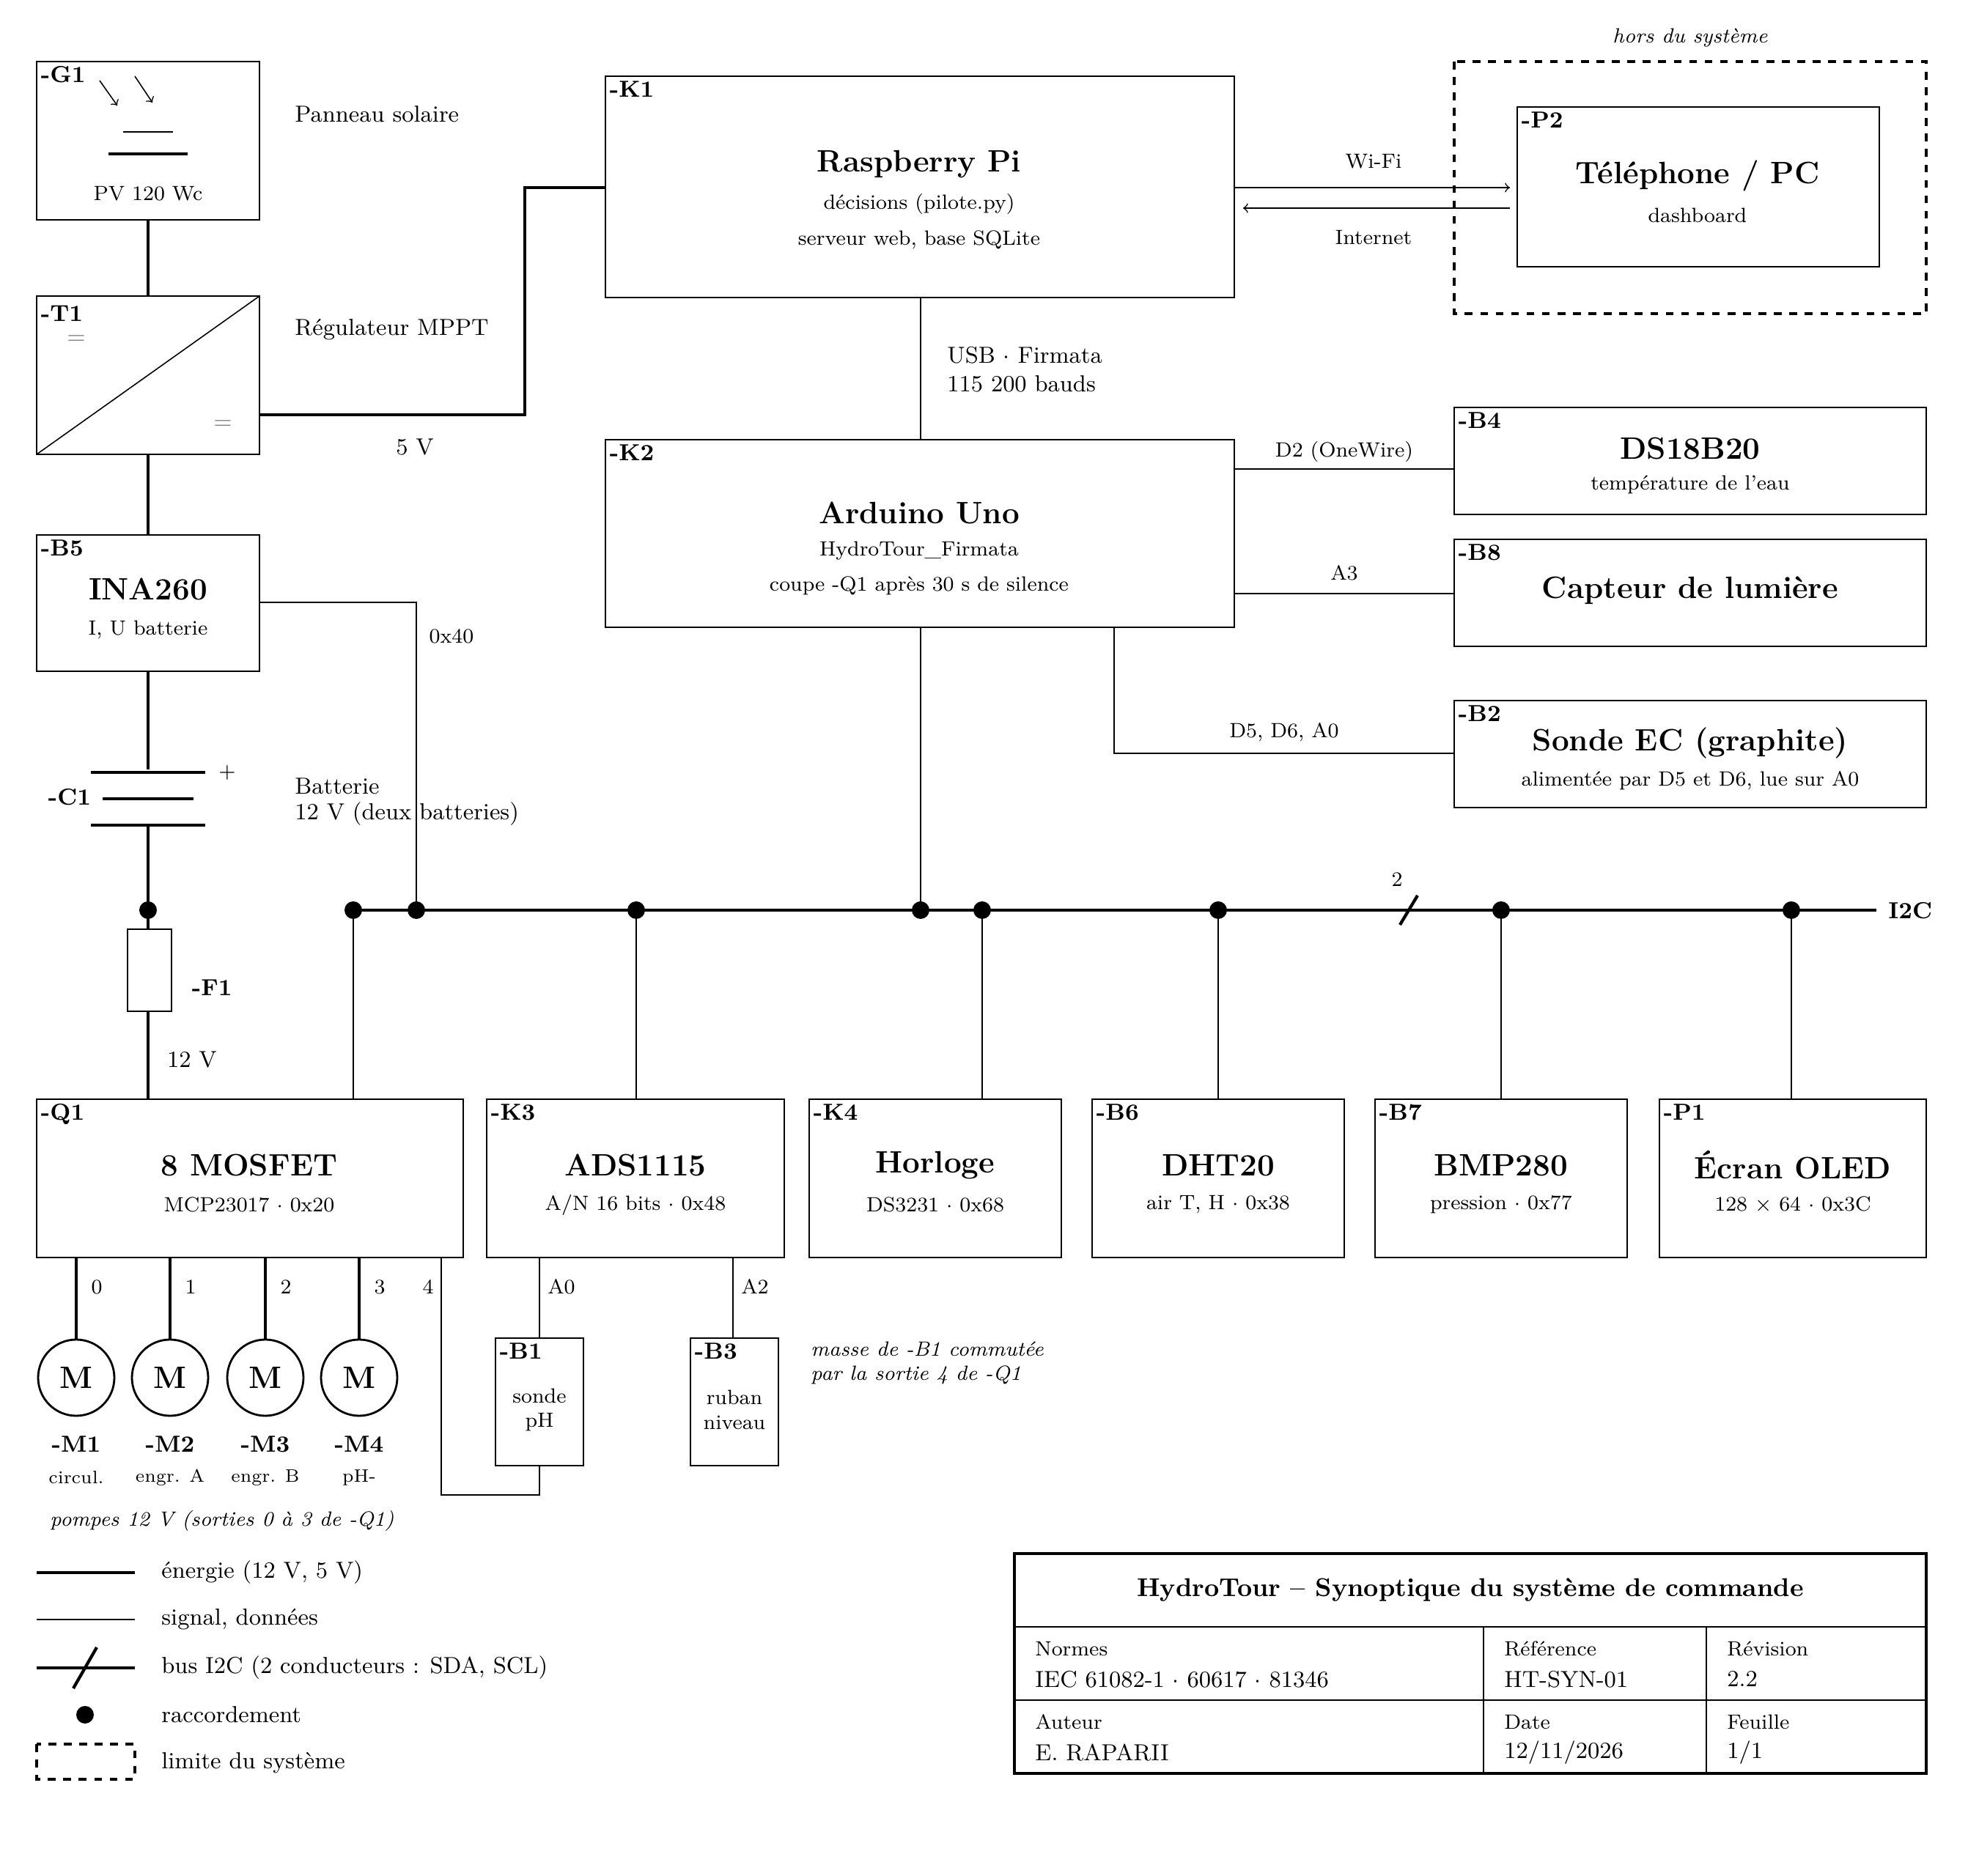
\includegraphics[width=\textwidth]{img/inf/f_synoptique.png}
\schemacap{synop}{Synoptique du système de commande, selon IEC 61082-1 (repères IEC 81346, symboles IEC 60617). Il représente le montage visé ; en attendant l'ADS1115, la sonde pH est branchée sur l'entrée A1 de -K2 (partie 8.2).}
\end{figure}

Ce synoptique montre les blocs. Pour câbler, il me faut le schéma électrique, que je dessine dans le style du schéma officiel de l'Arduino Uno : cadre à cases, fils verts, repères sur chaque composant et cartouche. Il tient sur une seule feuille vectorielle, présentée sur la page suivante en pleine page : alimentation et puissance (panneau, régulateur MPPT\ix{19}, INA260\ix{22}, batteries, fusibles, UBEC\ix{17}), commande (Raspberry Pi, Arduino, bus I2C\ix{12}, carte MOSFET\ix{15}, pompes) et capteurs, dont la sonde EC.

\schemapaysageC{eagle/schema_complet.pdf}{elcompl}{Schéma électrique complet de la tour (alimentation, commande, capteurs et sonde EC), sur une seule feuille.}

\subsubsection*{Les cartes électroniques}

Je cherche à comprendre ce que chaque carte sait faire avant de lui confier un rôle. Quatre cartes forment la chaîne qui va du programme jusqu'aux pompes : chacune compense une limite de la précédente. Le Raspberry ne sait pas lire une tension, l'Arduino la lit mais pas assez finement, et aucun des deux ne peut fournir le courant d'une pompe \qty{12}{V}.

\textbf{-K1 : Raspberry Pi.} Ce que c'est : un ordinateur complet de la taille d'une carte bancaire, sous Linux, avec Wi-Fi et carte mémoire. Son rôle : faire tourner le serveur en Python, prendre les décisions, garder l'historique des mesures et servir le dashboard. Il est alimenté en \qty{5}{V} et relié à l'Arduino par USB.

\textbf{-K2 : Arduino Uno.} Ce que c'est : une carte à microcontrôleur (ATmega328P, \qty{16}{MHz}, \qty{2}{Ko} de mémoire vive) qui lit et commande des broches électriques. Son rôle : faire l'interface entre le Raspberry et le matériel : bus I2C\ix{12}, sonde de température, capteur de lumière, sécurité des pompes. Elle dispose de 6 entrées analogiques, 14 broches numériques et d'un bus I2C\ix{12}.

\textbf{-Q1 : carte 8 MOSFET\ix{15} (Adafruit 6318).} Ce que c'est : huit interrupteurs électroniques (transistors MOSFET\ix{15}) commandés par une puce MCP23017 en I2C\ix{12}, avec une diode de protection et une LED par sortie. Son rôle : allumer et éteindre les quatre pompes \qty{12}{V} et l'alimentation des sondes pH et EC. Elle accepte de \qty{3}{V} à \qty{24}{V}, \qty{3,6}{A} par sortie, à l'adresse 0x20.

\textbf{-K3 : convertisseur ADS1115\ix{16}.} Ce que c'est : un convertisseur analogique-numérique à 4 entrées, beaucoup plus précis que celui de l'Arduino. Son rôle : transformer en nombres les tensions de la sonde pH et du ruban de niveau (la sonde EC est lue directement par l'Arduino). Il travaille sur 16 bits avec un pas de \qty{0,19}{mV}, à l'adresse 0x48.

\subsubsection*{Les capteurs}

Pour chaque capteur, je m'intéresse à son principe de mesure : c'est lui qui explique les précautions à prendre, comme l'étalonnage de la sonde pH, la correction en température de l'EC ou l'alternance entre les deux sondes. Les capteurs se répartissent en deux groupes : ceux de l'eau, qui servent à doser, et ceux de l'énergie et de l'air.

\textbf{Les capteurs de l'eau.}

\textbf{-B1 : sonde pH (DFRobot SEN0161-V2).} Une électrode de verre produit une petite tension qui varie d'environ \qty{59}{mV} par unité de pH. La carte qui l'accompagne l'amplifie et la décale : environ \qty{1,5}{V} à pH 7, et la tension monte quand l'eau devient plus acide. La sonde vieillit et doit être étalonnée dans deux solutions tampon (pH 7 et pH 4).

\naturecalc{théorie (formule démontrée, valeurs de fiches techniques et hypothèses ; rien de mesuré)}
\begin{demonstration}[pente de l'électrode de verre]
\resultat{\dfrac{RT\ln 10}{F} \approx \qty{59,16}{mV}\ \text{par unité de pH à \qty{25}{\celsius}}}
La tension de l'électrode varie comme le logarithme de l'activité des ions $\mathrm{H^+}$. Une variation d'une unité de pH multiplie cette activité par $10$, donc ajoute $\ln 10$ au logarithme. La tension varie alors de :
\[
\Delta U = \frac{R\,T}{F}\,\ln 10
\]
avec $R = \qty{8,314}{J/(mol.K)}$ la constante des gaz parfaits, $T = \qty{298,15}{K}$ la température absolue (\qty{25}{\celsius}) et $F = \qty{96485}{C/mol}$ la constante de Faraday. On calcule ligne par ligne :
\begin{align*}
R\,T &= \qty{8,314}{J/(mol.K)} \times \qty{298,15}{K} = \qty{2478,8}{J/mol}\\
R\,T\,\ln 10 &= \qty{2478,8}{J/mol} \times 2{,}3026 = \qty{5707,7}{J/mol}\\
\Delta U &= \frac{\qty{5707,7}{J/mol}}{\qty{96485}{C/mol}}\\
\Delta U &\approx \qty{0,05916}{V} \approx \qty{59,16}{mV}
\end{align*}
Je l'arrondis à \qty{59}{mV} par unité de pH dans le texte.
\end{demonstration}

\textbf{-B2 : sonde EC fabriquée (deux mines de graphite 4B).} Deux électrodes, ici deux mines de crayon en graphite montées dans un tube imprimé, font passer un courant alternatif dans l'eau. Plus l'eau contient de sels dissous, donc d'engrais, mieux elle conduit le courant. L'EC donne ainsi la quantité de nutriments disponibles. Je fabrique cette sonde moi-même parce que la commande de la sonde du commerce (DFRobot DFR0300) tarde à arriver (partie 7). Sa constante de cellule $K$ est estimée entre \qty{0,97}{cm^{-1}} et \qty{3,04}{cm^{-1}} (elle sera fixée à l'étalonnage) et elle couvre de \qtyrange{0,5}{3,0}{mS/cm}. Elle n'a pas de carte d'interface : l'Arduino la branche lui-même, par les broches D5 et D6 (courant alternatif, en série avec une résistance de \qty{330}{\ohm}), et lit la tension sur l'entrée A0. Elle dépend de la température, d'où la correction à \qty{25}{\celsius}, et elle s'étalonne avec deux solutions de KCl (partie 7.7). Elle n'est ni construite ni testée à ce jour.

\textbf{-B3 : ruban de niveau eTape\ix{23} (\qty{30}{cm}).} La pression de l'eau écrase l'enveloppe du ruban, qui court-circuite une partie de sa piste résistive : plus l'eau monte, plus sa résistance baisse (environ \qty{2000}{\ohm} à vide et \qty{400}{\ohm} plein). Monté en série avec une résistance de \qty{560}{\ohm}, il donne une tension lue par l'ADS1115\ix{16}.

\textbf{-B4 : sonde de température DS18B20\ix{24}.} Un capteur numérique étanche : il envoie directement la température sur un seul fil (protocole OneWire), avec un contrôle d'erreur. Sa précision est de \qty{\pm0,5}{\celsius}. La température de l'eau sert à corriger l'EC et à surveiller les racines.

\textbf{Les capteurs de l'énergie et de l'air.}

\textbf{-B5 : capteur de batterie INA260\ix{22}.} Le courant de la batterie traverse une très petite résistance de \qty{2}{m\ohm} placée dans le module ; la tension à ses bornes donne le courant, positif en charge, négatif en décharge. Il mesure aussi la tension de la batterie, au millivolt près. Le serveur en déduit le pourcentage de charge restant.

\textbf{-K4 : horloge DS1307.} Une horloge à pile qui garde l'heure quand tout est éteint. Sans Internet, le Raspberry ne connaît pas l'heure après une coupure : il la reprend sur cette horloge, pour que les mesures et le calendrier des légumes restent justes.

\textbf{-B6, -B7, -B8, -P1 : Sensor Kit Arduino.} Une carte qui regroupe plusieurs modules prêts à brancher : le DHT20\ix{24} (température et humidité de l'air), le BMP280 (pression de l'air), un capteur de lumière analogique et un écran OLED de $128 \times 64$ points qui affiche les mesures sur la tour.

\textbf{Pourquoi la lumière en \% ?} Le capteur de lumière du kit n'est pas étalonné : il donne une valeur relative, pas des lux. Je l'affiche donc en pourcentage de sa pleine échelle. Il sert surtout à savoir s'il y a du soleil pour relancer la pompe (partie 8.4).

\subsubsection*{Les pompes}

La tour utilise deux sortes de pompes, parce que les besoins sont opposés : déplacer beaucoup d'eau pour arroser, et verser quelques millilitres très précis pour doser. Je garde des pompes en \qty{12}{V} pour qu'elles fonctionnent directement sur la batterie solaire, sans onduleur.

\textbf{-M1 : pompe principale (circulation).} Une pompe immergée de \qty{12}{V} et \qty{19}{W}, prévue dans la nomenclature (jusqu'à \qty{800}{L/h} et \qty{5}{m} de hauteur). Elle remonte la solution nutritive en haut de la tour, d'où elle redescend le long des racines. C'est l'appareil qui consomme le plus : c'est elle qu'on coupe en premier quand la batterie baisse. Elle est sur la sortie 0 de la carte 8 MOSFET\ix{15}.

\textbf{-M2 à -M4 : pompes doseuses péristaltiques\ix{8}.} Des galets écrasent un tuyau souple en tournant et poussent devant eux un volume de liquide toujours identique. Le liquide ne touche que le tuyau, ce qui convient aux engrais et à l'acide. Leur débit d'au plus \qty{100}{mL/min} permet des doses de quelques millilitres : engrais A, engrais B et correcteur pH$-$. Elles sont sur les sorties 1, 2 et 3, en \qty{12}{V}, \qtyrange{0,2}{0,3}{A}.

\subsubsection*{Les programmes}

Je découpe le logiciel en plusieurs programmes, chacun avec une seule responsabilité. Ainsi, une modification des règles de dosage ne touche ni la communication avec l'Arduino ni le dashboard, et chaque morceau peut être testé séparément.

Le tableau suivant liste les programmes du système et le rôle de chacun.

\begin{table}[H]
\centering
\small
\begin{tabularx}{\textwidth}{|l|l|l|Y|}
\hline
\textbf{Programme} & \textbf{Où il tourne} & \textbf{Langage} & \textbf{Rôle} \\
\hline
\texttt{HydroTour\_Firmata} & Arduino & C++ & lire les capteurs et commander les sorties sur ordre ; sécurité de 30 s \\
\hline
\texttt{arduino.py} & Raspberry & Python & dialoguer avec l'Arduino, lire chaque capteur, allumer les pompes \\
\hline
\texttt{pilote.py} & Raspberry & Python & prendre les décisions : cycle, batterie, soleil, dosage, alertes \\
\hline
\texttt{server.py} & Raspberry & Python (Flask) & le serveur : boucle de mesure, base de données, site web \\
\hline
\texttt{hydrotour.html} & navigateur & HTML, JavaScript & le dashboard, avec la tour en 3D \\
\hline
\texttt{hydrotour.db} & Raspberry & SQLite & la base de données : mesures, réglages, stock, légume \\
\hline
\texttt{essai\_materiel.py} & Raspberry & Python & essai de tout le matériel avant la mise en route \\
\hline
\texttt{acces.py} & Raspberry & Python & page de connexion, captcha et réglage de l'identifiant et du mot de passe (partie 8.6) \\
\hline
\texttt{diagnostic.py} & Raspberry & Python & liste ce qui répond vraiment sur l'Arduino (partie 8.7) \\
\hline
\end{tabularx}
\caption{Les programmes du système.}
\end{table}

\subsubsection*{Le serveur}

Le serveur est le programme qui fait vivre la tour. J'ai besoin d'un programme qui tourne en permanence sur le Raspberry et qui fasse deux choses à la fois : piloter la tour sans interruption, et répondre au dashboard dès qu'on l'ouvre. Je choisis Python avec la bibliothèque Flask, simple et légère, qui suffit largement pour un seul utilisateur et fonctionne bien sur un Raspberry.

Un serveur est un programme qui attend des demandes et y répond. Celui de la tour est lancé automatiquement au démarrage du Raspberry par un service du système (partie 8.7). Il écoute sur deux ports : le 5000 pour les appareils du réseau de la maison, et le 5001, réservé à l'accès par Internet (partie 8.6). À l'intérieur, deux tâches tournent en parallèle :

\begin{itemize}
\item la \textbf{boucle de pilotage}, toutes les 10 s : elle lit les capteurs par l'Arduino, demande ses décisions au pilote, commande les pompes, enregistre la mesure dans la base et met à jour l'écran ;
\item le \textbf{serveur web} : il envoie la page du dashboard, puis répond à ses demandes (dernière mesure, historique, réglages, commandes manuelles).
\end{itemize}

Le schéma suivant montre comment la boucle de pilotage et le serveur web tournent en même temps dans le serveur.

\begin{figure}[H]
\centering
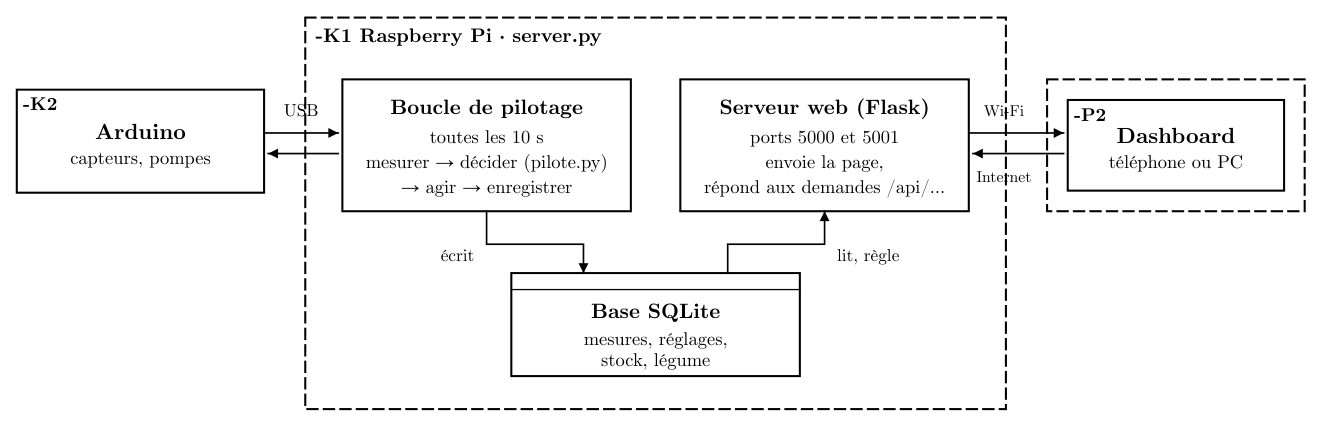
\includegraphics[width=0.95\textwidth]{img/inf/f_serveur.png}
\schemacap{serveur}{Le serveur : la boucle de pilotage et le serveur web tournent en même temps et partagent la même base de données.}
\end{figure}

Le dashboard dialogue avec le serveur par des adresses web simples, appelées API :

\begin{table}[H]
\centering
\small
\begin{tabularx}{\textwidth}{|l|Y|}
\hline
\textbf{Adresse} & \textbf{Ce qu'elle fait} \\
\hline
\texttt{/api/latest} & dernière mesure, état des pompes, alertes et journal du pilote \\
\hline
\texttt{/api/history} & historique des mesures pour les courbes et l'export en tableur \\
\hline
\texttt{/api/pompe} & commande manuelle : démarrer ou arrêter la circulation, dose de quelques secondes \\
\hline
\texttt{/api/pilotage} & lire ou changer les réglages : automatique, cycle, seuils de batterie \\
\hline
\texttt{/api/culture} & légume cultivé et date de plantation, d'où le serveur déduit les cibles \\
\hline
\texttt{/api/etalonner} & enregistrer l'étalonnage du pH (7 et 4) et du réservoir (vide et plein) \\
\hline
\texttt{/api/stock}, \texttt{/api/batterie} & litres d'engrais disponibles ; capacité et tension de la batterie \\
\hline
\texttt{/connexion}, \texttt{/api/acces} & page de connexion avec son captcha ; changer l'identifiant et le mot de passe (partie 8.6) \\
\hline
\end{tabularx}
\caption{Les adresses de l'API.}
\end{table}

Le serveur s'occupe aussi de l'heure : une fois par heure, il remet l'horloge à pile à l'heure d'Internet si le Raspberry y a accès, ou prend l'heure de l'horloge dans le cas contraire. Enfin, quand on l'arrête, il coupe toutes les pompes avant de se fermer.

\subsubsection*{Le dashboard}

Je veux pouvoir surveiller et régler la tour sans être devant, depuis un simple téléphone. Plutôt qu'une application à installer, je choisis une page web : elle s'ouvre dans n'importe quel navigateur, à l'adresse \texttt{http://<ip-du-raspberry>:5000}, et se met à jour toute seule toutes les 10 secondes. Depuis novembre, on peut aussi l'ouvrir depuis n'importe où, par une adresse en \texttt{https://...ts.net} : une page de connexion protège alors l'accès (partie 8.6).

Le dashboard est organisé en quatre onglets : Mesures (les valeurs, leurs cibles et leurs courbes), Installation (la tour en 3D, le calendrier du légume et les pompes), Journal (ce que la tour a fait et pourquoi) et Paramètres (accès, légume, batterie, pilotage, étalonnage). Sans serveur, il passe en mode démonstration avec des valeurs simulées. Il est présenté en détail, avec des captures, dans la partie 8.5.

\subsubsection*{Des mesures en alternance}

En préparant le câblage, je relève dans la nomenclature que la sonde EC perturbe la sonde pH. Cette contrainte change la façon de mesurer, c'est pourquoi je la présente dès maintenant. Pour mesurer, la sonde EC envoie un courant dans l'eau. Tant qu'elle est alimentée, ce courant fausse la sonde pH plongée dans le même réservoir. Les deux sondes ne sont donc jamais allumées en même temps : le pH est lu toutes les 10 s, sonde EC éteinte, et l'EC une fois par minute, pendant 2 s, sonde pH éteinte. Le détail du montage et du déroulement est donné dans la partie 8.2.

